\documentclass{standalone}
\usepackage{tikz}
\usetikzlibrary{shapes}
%\usetikzlibrary{arrows.meta} 
%\tikzset{>={Latex[width=4mm,length=4mm]}}

\usetikzlibrary{shapes}

\tikzset{My Arrow Style/.style={single arrow, fill=gray, anchor=base, align=center,text width=1.8cm}}
\newcommand{\MyArrow}[2][]{\tikz[baseline] \node [My Arrow Style,#1] {#2};}

\begin{document}
	\begin{tikzpicture}
		\node at (0,0) {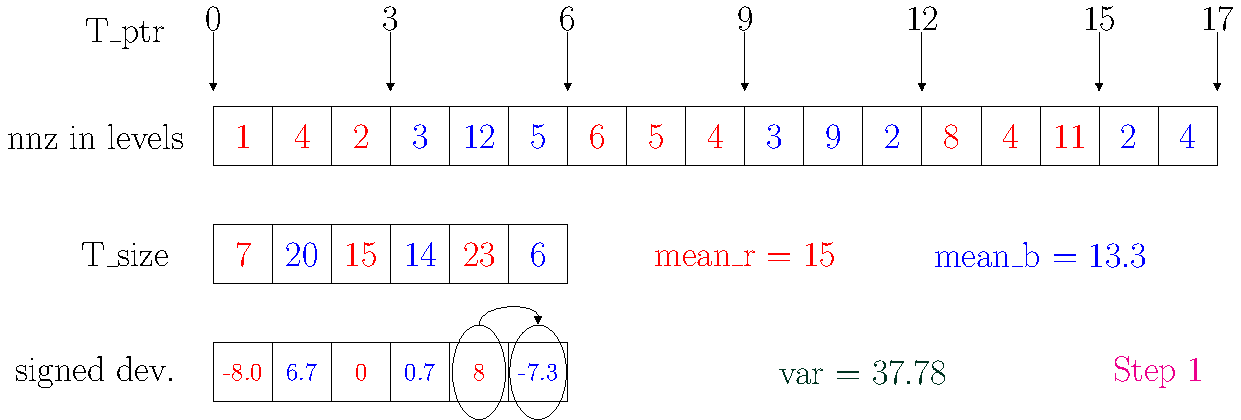
\includegraphics{lb_1}};
		\node at (22,0) {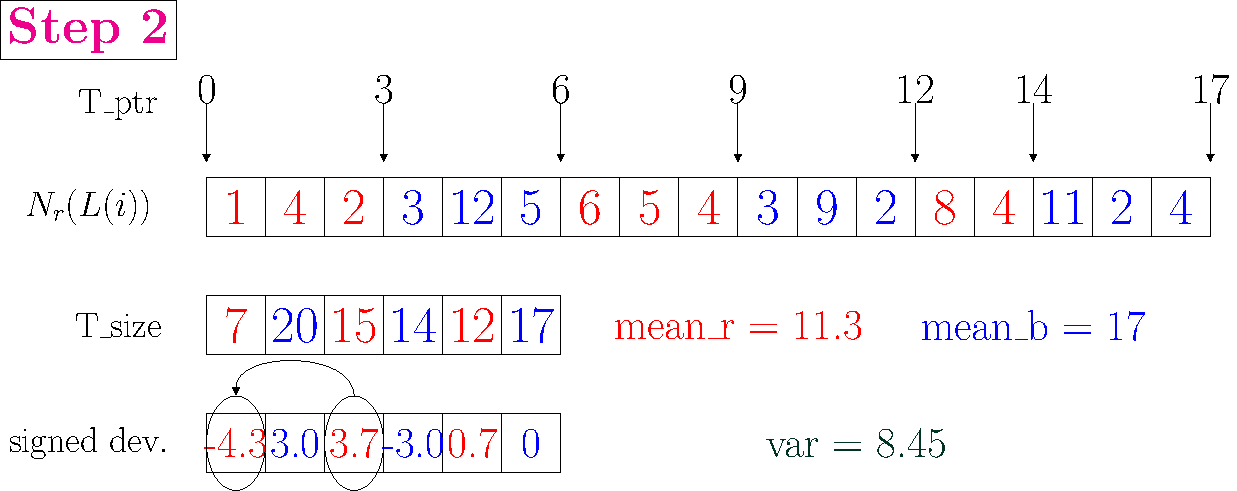
\includegraphics{lb_2}};
		\node at (22,-8.5) {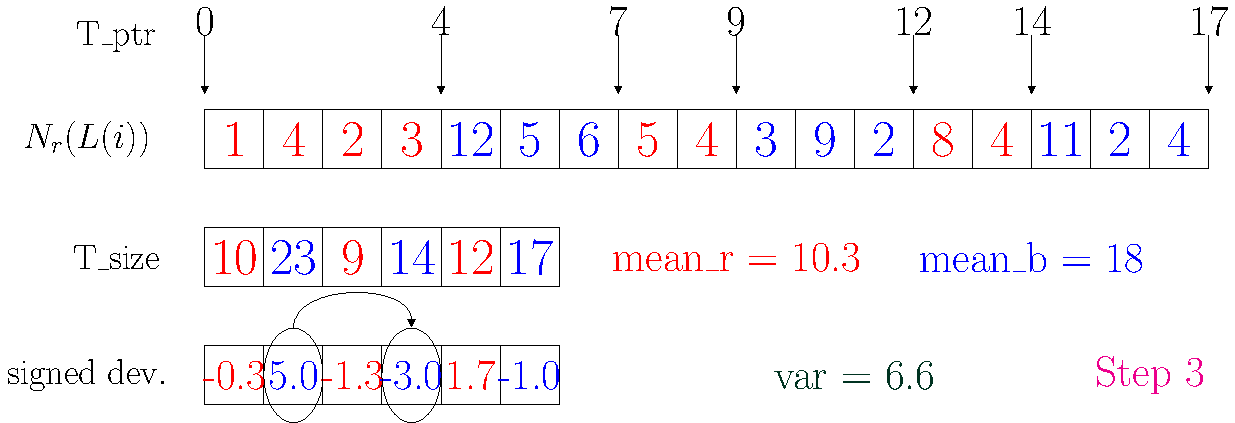
\includegraphics{lb_3}};
		\node at (0,-8.5) {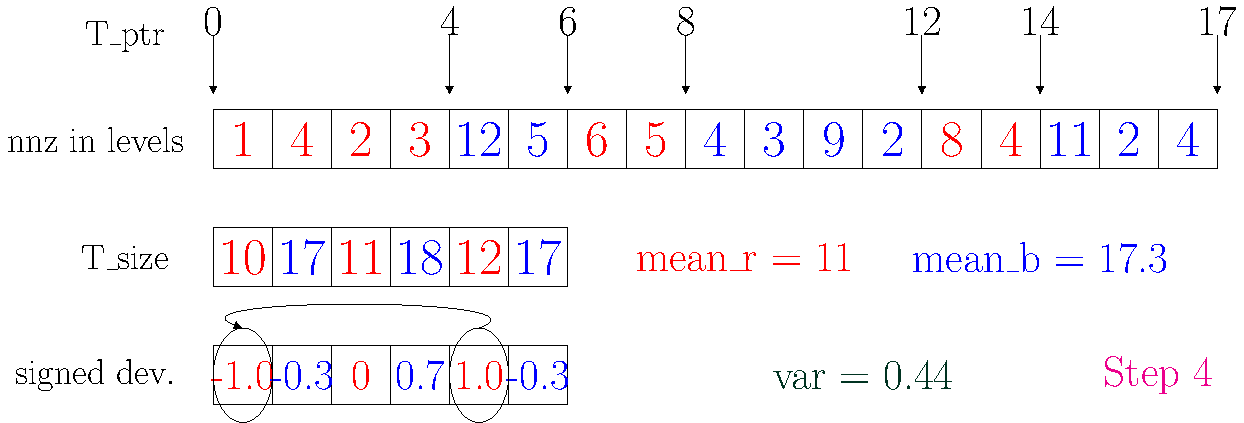
\includegraphics{lb_4}};
		\draw (-10.5,-3.8) -- (32.5,-3.8);
		\draw (11,3.5) -- (11,-10.8);
		

		\node at (11,-1) {\MyArrow{}};
		\node[rotate=-90] at (28,-3.5) {\MyArrow{}};
		\node[rotate=180] at (11,-8) {\MyArrow{}};
	\end{tikzpicture}
\end{document}